\documentclass[wcp]{jmlr}

\usepackage{booktabs}
\usepackage{array}
\setlength{\bibsep}{0pt}

\newcommand{\tablenote}[1]{%
  \vspace{4pt}%
  \begin{minipage}{0.95\linewidth}%
    \footnotesize\raggedright\emph{Note.}~#1\par%
  \end{minipage}%
}

\jmlrvolume{}
\jmlryear{2026}
\jmlrworkshop{ACML 2026}
\editor{}

\title{Don't Overthink It: Random Forests Outperform Deep Learning for Drug-Target Binding Affinity}

\author{\phantom{Anonymous}}
\date{}

\begin{document}
\maketitle

\begin{abstract}
Deep learning architectures---graph neural networks, transformers, and attention-based models---are widely considered the frontier for protein-ligand binding affinity prediction. We test this claim with the largest systematic benchmark to date: 16 model families, 350 experiments (331 under Bemis--Murcko scaffold split; remainder cross-dataset and zero-shot), with multi-seed validation and bootstrap confidence intervals. A Random Forest with 1024-bit ECFP4 fingerprints and 20-feature amino acid composition achieves test RMSE of 1.006 (Pearson $R = 0.747$), outperforming every purely deep learning architecture tested. Model family accounts for 47\% of performance variance by RF importance (72\% of explainable variance by Type~II ANOVA); protein representation contributes 8\% and is not statistically significant beyond what family and ligand already explain. Pretrained protein language model embeddings (ESM-2) improve deep learning models by 10--17\% but provide negligible benefit to tree ensembles, and scaling ESM-2 from 8M to 650M parameters yields no improvement. Our results suggest that resources should shift toward representation quality and rigorous evaluation rather than architectural complexity.
\end{abstract}

\begin{keywords}
Binding affinity prediction, benchmark, scaffold split, deep learning, random forest, protein language models, molecular fingerprints
\end{keywords}

\section{Introduction}

Deep learning has transformed computational drug discovery. Graph neural networks (GNNs) encode molecular topology directly~\citep{kipf2017gcn,gilmer2017mpnn}, protein language models (PLMs) produce per-residue embeddings from sequence~\citep{lin2023esm2}, and chemical language models enable generative design and property prediction from string representations~\citep{ozcelik2024s4,ozcelik2024hitchhiker}. Cross-attention architectures model protein-ligand interactions at atomic resolution~\citep{capla2023,cucco2026molxprot}. Each new architecture reports improvements on standard benchmarks, creating a narrative of steady progress.

But how much of this progress is real? The free energy community has long recognized that rigorous benchmarking requires careful attention to statistical uncertainty~\citep{shirts2008mbar,paliwal2011benchmark} and standardized protocols~\citep{mey2024benchmark}. The SAMPL blind challenges~\citep{rizzi2020sampl6} showed that even with identical parameters, predictions can differ by 0.3--1.0~kcal/mol, a margin that demands controlled comparisons. These lessons have not fully transferred to the ML community. Random splits---still used by many papers including MolXProt~\citep{cucco2026molxprot}---allow compounds sharing the same scaffold to appear in both training and test sets. Models memorize scaffold-affinity associations rather than learning transferable binding physics. Under scaffold-based splits, the picture changes~\citep{balm2024,landrum2024ic50}: fingerprint-based tree ensembles match or exceed deep learning models on several benchmarks~\citep{balm2024,gorantla2023proteins,gorantla2024benchmarking}.

This raises an uncomfortable question: has the field been over-investing in architectural complexity while under-investing in rigorous evaluation? We present the most extensive empirical answer to date: 350 experiments spanning 16 model families---linear, tree ensembles (RF, XGBoost, LightGBM), multi-layer perceptrons, CNN-based, LSTM and Mamba, transformers, graph neural networks (GCN, GAT), bidirectional cross-attention (BiCA, BiCA~v2/ChemCross), Gaussian Processes (Tanimoto, RBF, Mat\'ern, RQ kernels), and PSICHIC~\citep{hao2024psichic}. After selecting the best-completed run per configuration, 286 unique seed-42 experiments form the primary leaderboard pool; the remaining experiments cover multi-seed validation, cross-dataset transfer, and zero-shot evaluation. Every experiment in the primary leaderboard uses the same BindingDB\_filtered dataset under a Bemis--Murcko scaffold split (seed 42, with multi-seed validation at 123 and 456); cross-dataset experiments use LeakyPDB, Mpro, USP7, and ASAP Polaris benchmarks as noted in Section~\ref{sec:cross_dataset}. All results are evaluated under the same metrics (RMSE, Pearson $R$, Spearman $\rho$) and logged with bootstrap 95\% confidence intervals.

Our central finding is unambiguous: a Random Forest with ECFP4 fingerprints and amino acid composition outperforms every deep learning architecture tested. The simplest model wins decisively. Model family accounts for 47\% of performance variance by RF importance (72\% of explainable variance by Type~II ANOVA); protein representation contributes 8\% and is not statistically significant. We identify two additional findings: (1) pretrained protein representations (ESM-2) improve deep learning by 10--17\% but provide negligible benefit to tree ensembles; (2) scaling ESM-2 from 8M to 650M parameters yields no improvement.

\section{Related Work}

\subsection{Deep Learning for Binding Affinity Prediction}

Predicting protein-ligand binding has seen many approaches over the last 50 years. Docking using physics-based scoring functions~\citep{kitchen2004docking} and classical QSAR models use algorithms such as Random Forest on molecular fingerprints---particularly Extended Connectivity Fingerprints (ECFP)~\citep{rogers2010ecfp}---encoding circular substructures as bit vectors~\citep{svetnik2003rf}. Deep learning has proliferated for Drug-Target Binding Affinity (DTA) since DeepDTA~\citep{ozturk2018deepdta}, exploring three directions: graph-based methods (GCN~\citep{kipf2017gcn}, GAT~\citep{velickovic2018gat}, MPNN~\citep{gilmer2017mpnn}); attention-based fusion through cross-attention (CAPLA~\citep{capla2023}, CoaDTI~\citep{coadti2022}) or bilinear attention (DrugBAN~\citep{attentionmgt2024}); and pretrained representations from protein language models (ESM-2~\citep{lin2023esm2}) and chemical language models (ChemBERTa~\citep{ahmad2022chemberta}, S4~\citep{ozcelik2024s4}). MolXProt~\citep{cucco2026molxprot} combines GNN ligand encoding, ESM-2 embeddings, and bidirectional cross-attention.

Interpretability has received increasing scrutiny~\citep{yang2019concepts,jimenez2021ai}, with Lavecchia~\citep{lavecchia2025xai} identifying three requirements for credible claims: ground-truth validation, quantitative fidelity, and explicit handling of shortcut learning. Methodological advances include SHAP-based attribution~\citep{danel2020shap}, substructure masking for GNNs~\citep{wang2023sme}, gradient-weighted activation mapping~\citep{yang2022mgraphdta}, and explainable active learning frameworks that integrate uncertainty quantification with interpretable model outputs~\citep{srivastava2026explainable}. Despite this, most published DTA architectures report only qualitative attention visualizations.

\subsection{The Importance of Evaluation Protocol}

The choice of data split critically affects reported performance. Time-split validation produces substantially different rankings than random splits~\citep{sheridan2013timesplit}. The free energy community has long led on rigorous protocols: SAMPL blind challenges~\citep{rizzi2020sampl6} and community best-practice guidelines~\citep{mey2024benchmark} established standards for binding affinity assessment. On the ML side, BALM~\citep{balm2024} established scaffold-split evaluation and a curated BindingDB benchmark as community infrastructure for binding affinity assessment. Systematic evaluations of deep learning methods~\citep{gorantla2023proteins} and active learning protocols~\citep{gorantla2024benchmarking} have further highlighted the importance of rigorous experimental design~\citep{landrum2024ic50}.

\subsection{Protein Representations}

Protein language models, particularly ESM-2~\citep{lin2023esm2}, have become the de facto standard for protein featurization~\citep{singh2026explainable,singh2026antibody,prabakaran2026quantifying}. Trained on 250 million sequences, ESM-2 produces per-residue embeddings encoding structural and functional information. Variants range from 8M to 15B parameters. ProtTrans~\citep{elnaggar2022prottrans} provides a complementary 256-dim representation. Our benchmark systematically tests these across architectures, revealing architecture-dependent benefits: deep models gain 10--17\%, tree ensembles gain nothing.

\subsection{Benchmarking and Meta-Analysis}

Large-scale benchmarks have driven progress in computer vision (ImageNet) and NLP (GLUE). In computational chemistry, MoleculeNet and Therapeutics Data Commons standardized evaluation. The BALM benchmark~\citep{balm2024} provides a scaffold-split framework for binding affinity. Our work extends this with the largest controlled comparison of model architectures for DTA.

\section{Methods}

\subsection{Dataset and Split}

We use the BindingDB\_filtered dataset from the BALM benchmark~\citep{balm2024}, comprising 24,700 protein-ligand pairs with experimentally measured dissociation constants ($K_d$). All affinities are converted to $\text{p}K_d = 9 - \log_{10}(K_d\ [\text{nM}])$. The primary evaluation uses a Bemis--Murcko scaffold split~\citep{bemis1996murcko} with fixed random seed 42: 17,312 training pairs, 2,673 validation pairs, and 4,715 test pairs. Multi-seed validation uses seeds 123 and 456.

\subsection{Molecular Representations}

We evaluate 16 ligand representations spanning four categories: (1) classical fingerprints---ECFP4 (1024-bit), ECFP6 (1024-bit), MACCS (167-bit); (2) pretrained embeddings---ChemBERTa-2 variants (5M/77M/100M parameters, base 600-dim); (3) molecular graphs---78-dim atom features with 10-dim bond features for GNN models; (4) topological descriptors---100$\times$100 distance matrices and 200 RDKit descriptors. For protein representations, we evaluate 8 options: AAC (20-dim), dipeptide composition (400-dim), k-mer hashing (3-mers, 8000-dim), ESM-2 variants (8M/320-dim, 35M/480-dim, 150M/640-dim, 650M/1280-dim per residue), ESMC (300M/960-dim), and ProtTrans (256-dim). For flat-vector models, pretrained per-residue embeddings are mean-pooled across the sequence dimension.

\subsection{Model Families}

Sixteen model families are evaluated, spanning classical machine learning and contemporary deep learning:

\begin{table*}[t]
\centering
\small
\caption{Evaluated model families and experiment counts.}
\label{tab:families}
\begin{tabular}{@{}>{\raggedright\arraybackslash}p{0.14\textwidth} >{\raggedright\arraybackslash}p{0.55\textwidth} >{\centering\arraybackslash}p{0.12\textwidth}@{}}
\toprule
\textbf{Category} & \textbf{Families} & \textbf{\# Exp.} \\
\midrule
Classical & Linear (Ridge); tree ensembles (RF, XGBoost, LightGBM); Gaussian processes (Tanimoto, RBF, Mat\'ern, RQ) & 123 \\
Feed-forward & MLP (shallow, medium, deep) & 63 \\
Sequence & LSTM; sequence Transformer; Mamba & 60 \\
Convolutional & 1D CNN; distance-matrix CNN & 20 \\
Graph-based & GCN; GAT & 25 \\
Cross-attention & BiCA (flat); BiCA v2 / ChemCross (sequence) & 57 \\
External & PSICHIC (zero-shot and fine-tuned) & 2 \\
\bottomrule
\end{tabular}
\end{table*}

All models are trained with early stopping (patience = 20 on validation RMSE). Primary metric: test RMSE (p$K_d$). Secondary: Pearson $R$, Spearman $\rho$. Bootstrap 95\% confidence intervals (1,000 resamples) are reported for all family representatives. ESM-2 and ChemBERTa encoders are frozen to ensure representation parity; this conservative choice may understate deep models that benefit from end-to-end adaptation (we report PLM fine-tuning experiments in Section~\ref{sec:architecture}); fine-tuning the top 3 ESM-2 layers for MLP did not improve over frozen encoders. Training on a single NVIDIA A4000 GPU (16~GB); tree models on CPU. Protein sequences truncated to $L_\text{prot}=512$ ($>$99\% coverage), ligand tokens to $L_\text{lig}=256$. Key hyperparameters summarized in Table~\ref{tab:hparams}; full search grids are provided in the code repository.

\begin{table*}[t]
\centering
\small
\caption{Hyperparameter Settings Per Model Family}
\label{tab:hparams}
\begin{tabular}{lp{5.3cm}p{5.3cm}}
\toprule
\textbf{Family} & \textbf{Key Hyperparameters} & \textbf{Tuning Strategy} \\
\midrule
RF & 500 trees, max\_depth=20, min\_samples\_split=2, max\_features=$\sqrt{d}$ & Fixed (strong defaults) \\
XGBoost & 500 trees, max\_depth=8, lr=0.1, subsample=0.8 & Fixed (standard config) \\
LightGBM & 500 trees, max\_depth=8, lr=0.1, num\_leaves=31 & Fixed (standard config) \\
MLP & 2--4 layers, 256--512 hidden, lr=1e-3, dropout=0.3, AdamW & Fixed architecture variants \\
GCN/GAT & 3 layers, hidden=128, lr=1e-3, dropout=0.3, AdamW & Fixed (literature standard) \\
LSTM/Transformer & 2 layers, hidden=256, lr=1e-3, dropout=0.3, AdamW & Fixed architecture variants \\
BiCA/ChemCross & 2 cross-attn blocks, 8 heads, $d_\text{hidden}$=256, lr=1e-3, AdamW & Fixed (matched to MLP) \\
\bottomrule
\end{tabular}
\tablenote{%
  We acknowledge that fixed hyperparameters favor tree ensembles, which are robust to default settings.
  Deep models may benefit from additional tuning.
  Full search grids are provided in the code repository.
}
\end{table*}

\subsection{Protein Encoding Validation}
\label{sec:protein_encoding}

Does the protein feature carry genuine chemical information, or does the model simply memorize which target each compound binds to? We compared two protein encodings under identical conditions: amino acid composition (AAC, 20-dim), which encodes real chemical properties, and a 10-bit binary representation of the target's integer ID (\texttt{target\_binary}), which carries zero chemical meaning but allows the model to distinguish targets. Both use ECFP4 fingerprints and an RF regressor (200 trees, max\_depth=20) under Bemis--Murcko scaffold split across three seeds (42, 123, 456).

We evaluate using Fisher $z$-transformed per-target Pearson correlation~\citep{balm2024}, which gives equal weight to each protein target regardless of compound count. Table~\ref{tab:fisher_ablation} reports the results. AAC achieves Fisher $r = 0.49 \pm 0.05$ (mean $\pm$ std), substantially above \texttt{target\_binary} ($0.33 \pm 0.06$). AAC outperforms on every metric across all three seeds. The model extracts real chemical signal from amino acid composition, not just target identity. The Fisher $r$ is substantially lower than the Global $r$ (0.49 vs.\ 0.70 for AAC), revealing that performance concentrates on large, well-characterized targets---a pattern invisible under global metrics.

\begin{table}[t]
\centering
\footnotesize
\setlength{\tabcolsep}{2pt}
\caption{Protein encoding ablation with Fisher per-target evaluation.}
\label{tab:fisher_ablation}
\begin{tabular}{@{}lccc@{}}
\toprule
\textbf{Encoding} & \textbf{RMSE} & \textbf{Global $r$} & \textbf{Fisher $r$} \\
\midrule
AAC & 1.06 $\pm$ 0.04 & 0.70 $\pm$ 0.04 & 0.49 $\pm$ 0.05 \\
Binary ID & 1.30 $\pm$ 0.05 & 0.47 $\pm$ 0.08 & 0.33 $\pm$ 0.06 \\
\bottomrule
\end{tabular}
\tablenote{%
  Values are mean $\pm$ standard deviation across seeds 42, 123, and 456; Binary ID denotes \texttt{target\_binary}.
  Global $r$ weights compounds equally; Fisher $r$ weights protein targets equally using a Fisher $z$-transform.
}
\end{table}

Finally, we tested zero-shot generalization: the RF is trained on full BindingDB and evaluated directly on entirely unseen proteins (USP7, MPro) without retraining. For \texttt{target\_binary}, unseen targets receive an all-zero vector. Table~\ref{tab:zeroshot} reports the results.

\begin{table}[t]
\centering
\footnotesize
\caption{Zero-shot generalization to unseen proteins (RF + ECFP4, trained on BindingDB).}
\label{tab:zeroshot}
\begin{tabular}{@{}lrrrr@{}}
\toprule
\textbf{Encoding} & \textbf{USP7 RMSE} & \textbf{USP7 $R$} & \textbf{Mpro RMSE} & \textbf{Mpro $R$} \\
\midrule
AAC (20-dim)          & 1.381 & 0.38  & 1.565 & $-$0.01 \\
Binary ID (10-bit)    & 1.244 & 0.34  & 1.551 & $-$0.02 \\
ESM-2 8M (320-dim)    & 1.238 & 0.58  & 1.559 & $-$0.04 \\
\bottomrule
\end{tabular}
\tablenote{%
  Models trained on BindingDB\_filtered (seed 42), tested directly on USP7 and Mpro without retraining.
  \texttt{target\_binary} uses an all-zero vector for unseen targets.
}
\end{table}

ESM-2 provides a clear boost on USP7 (Pearson $R$ from 0.38 to 0.58), confirming that pretrained protein embeddings capture cross-proteome signal that simple amino acid counts miss. But Mpro remains near random for all three encodings. Even ESM-2 cannot transfer to targets that lie genuinely out of distribution relative to the BindingDB training proteins. This is consistent with BALM's finding that frozen PLM features alone are insufficient for zero-shot binding affinity~\citep{balm2024}; parameter-efficient fine-tuning or learned alignment between protein and ligand spaces is needed for true target-agnostic prediction. The key takeaway is that ESM-2 helps where there is shared proteome structure, but some targets require more than frozen features can provide.

\section{Results}

\subsection{Tree Ensembles Dominate the Scaffold-Split Leaderboard}

We first evaluate whether strong ligand-centric baselines are competitive under Bemis--Murcko scaffold splitting. Table~\ref{tab:leaderboard} presents the top-performing models ranked by test RMSE. The top 10 positions are occupied entirely by tree-based models. Random Forest with ECFP4 fingerprints and 20-dim amino acid composition achieves the best overall performance (RMSE = 1.006, Pearson $R = 0.747$, Spearman $\rho = 0.674$). The best \emph{pure} deep learning model---an MLP with ChemBERTa-5M ligand embeddings and ESM-2 8M protein embeddings---achieves RMSE = 1.074 at rank 33, representing a 6.8\% degradation relative to RF. Ranks 3--10 are also tree-based models (XGBoost, LightGBM) but use pretrained embeddings (ChemBERTa, ESM-2) as input features. These hybrids combine classical learners with deep representations; we analyze them separately from pure deep learning architectures.

\begin{table*}[t]
\centering
\small
\caption{Top-15 Test RMSE Leaderboard (Bemis--Murcko scaffold split, seed 42, $N=4{,}715$)}
\label{tab:leaderboard}
\begin{tabular}{lllrr}
\toprule
\textbf{Rank} & \textbf{Model} & \textbf{Representations} & \textbf{RMSE} & \textbf{Pearson $R$} \\
\midrule
 1 & RF              & ECFP4 + AAC                  & 1.006 & 0.747 \\
 2 & RF              & ECFP4 + Dipeptide            & 1.019 & 0.739 \\
 3 & XGBoost         & ChemBERTa-5M + ESM-2 650M    & 1.043 & 0.724 \\
 4 & XGBoost         & ChemBERTa-5M + ESM-2 35M     & 1.047 & 0.722 \\
 5 & XGBoost         & ECFP4 + ESM-2 8M             & 1.048 & 0.721 \\
 6 & XGBoost         & ChemBERTa-600 + ESM-2 650M   & 1.052 & 0.718 \\
 7 & LightGBM        & ECFP4 + AAC                  & 1.053 & 0.720 \\
 8 & XGBoost         & ChemBERTa-5M + ESM-2 8M      & 1.055 & 0.717 \\
 9 & XGBoost         & ChemBERTa-5M + ESMC 300M     & 1.059 & 0.713 \\
10 & XGBoost         & ChemBERTa-600 + ESMC 300M    & 1.063 & 0.711 \\
\midrule
\multicolumn{5}{c}{\textit{Best non-tree (deep learning) models}} \\
33 & MLP             & ChemBERTa-5M + ESM-2 8M       & 1.074 & 0.716 \\
38 & MLP             & ChemBERTa-77M + ESM-2 8M      & 1.080 & 0.710 \\
44 & MLP             & ChemBERTa-600 + ESM-2 650M    & 1.090 & 0.705 \\
50 & BiCA (flat)     & ChemBERTa-5M + ESMC 300M      & 1.102 & 0.702 \\
76 & BiCA v2 (seq)   & ChemBERTa + ESM-2 35M          & 1.132 & 0.681 \\
-- & Best GAT (GNN)  & MolGraph + ESM-2 650M         & 1.194 & 0.643 \\
-- & Best LSTM        & BPE + BPE                    & 1.146 & 0.660 \\
-- & PSICHIC (ft)    & Physicochemical               & 1.176 & 0.631 \\
-- & GP (RQ kernel)   & ECFP4                          & 1.179 & 0.628 \\
\bottomrule
\end{tabular}
\end{table*}

Several patterns stand out. Tree models occupy all 10 of the top 10 positions. Pretrained protein embeddings (ESM-2, ESMC) appear in the top-performing deep learning models but not in the top tree models, which use simple AAC or dipeptide features. The RMSE spread within the top 10 is narrow (1.006--1.063). Many configurations converge to similar predictive performance given strong representations. Across three independent scaffold seeds (42, 123, 456), RF + ECFP4 + AAC achieves mean RMSE of $1.062 \pm 0.036$ (200 trees, max\_depth=20), confirming the result is robust to the choice of scaffold partition.

Gaussian Process (GP) models---the standard virtual screening baseline---were evaluated with four kernels (Tanimoto, RBF, Mat\'ern 5/2, Rational Quadratic) on ECFP4 fingerprints. The best configuration (RQ kernel) achieves test RMSE = 1.179 (Pearson $R = 0.628$), trailing RF + ECFP4 + AAC by 17\%. Adding protein features does not improve GP predictions: AAC is neutral (RBF kernel RMSE unchanged at 1.238), while ESM-2 embeddings degrade performance (ESM-2 8M: RMSE = 1.439; 35M: RMSE = 1.492), as high-dimensional protein vectors dominate the RBF distance and drown the fingerprint signal. GP models rank below all tree ensembles, consistent with the broader pattern.

Table~\ref{tab:bs_ci} reports the best RMSE observed within each model family together with bootstrap 95\% confidence intervals for the within-family RMSE distribution. The tree-family interval sits entirely below the MLP interval. The advantage is not a single lucky run.

\begin{table*}[t]
\centering
\small
\caption{Family-Level RMSE Summary and Bootstrap 95\% Confidence Intervals}
\label{tab:bs_ci}
\begin{tabular}{lccc}
\toprule
\textbf{Family} & \textbf{Best RMSE} & \textbf{Family RMSE 95\% CI} & \textbf{\# Exps} \\
\midrule
Tree        & 1.006 & [1.070, 1.100] & 46 \\
MLP         & 1.074 & [1.148, 1.467] & 46 \\
BiCA        & 1.102 & [1.184, 1.214] & 48 \\
CNN         & 1.109 & [1.210, 1.305] & 20 \\
Transformer & 1.119 & [1.200, 1.241] & 44 \\
LSTM        & 1.146 & [1.176, 1.232] & 9 \\
Mamba       & 1.158 & [1.171, 1.210] & 7 \\
GP          & 1.179 & [1.208, 1.375] & 7 \\
GAT         & 1.194 & [1.221, 1.278] & 12 \\
GCN         & 1.202 & [1.214, 1.282] & 11 \\
Linear      & 1.254 & [1.394, 1.538] & 35 \\
\bottomrule
\end{tabular}
\tablenote{%
  CIs are bootstrap 95\% intervals over the \emph{mean} RMSE within each model family
  (1,000 resamples, family mean as the target statistic), computed from unique
  seed-42 experiments (best run retained per experiment\_id; $N=286$ total).
  Only families with $\geq$7 experiments are shown.
}
\end{table*}

\begin{figure*}[t]
    \centering
    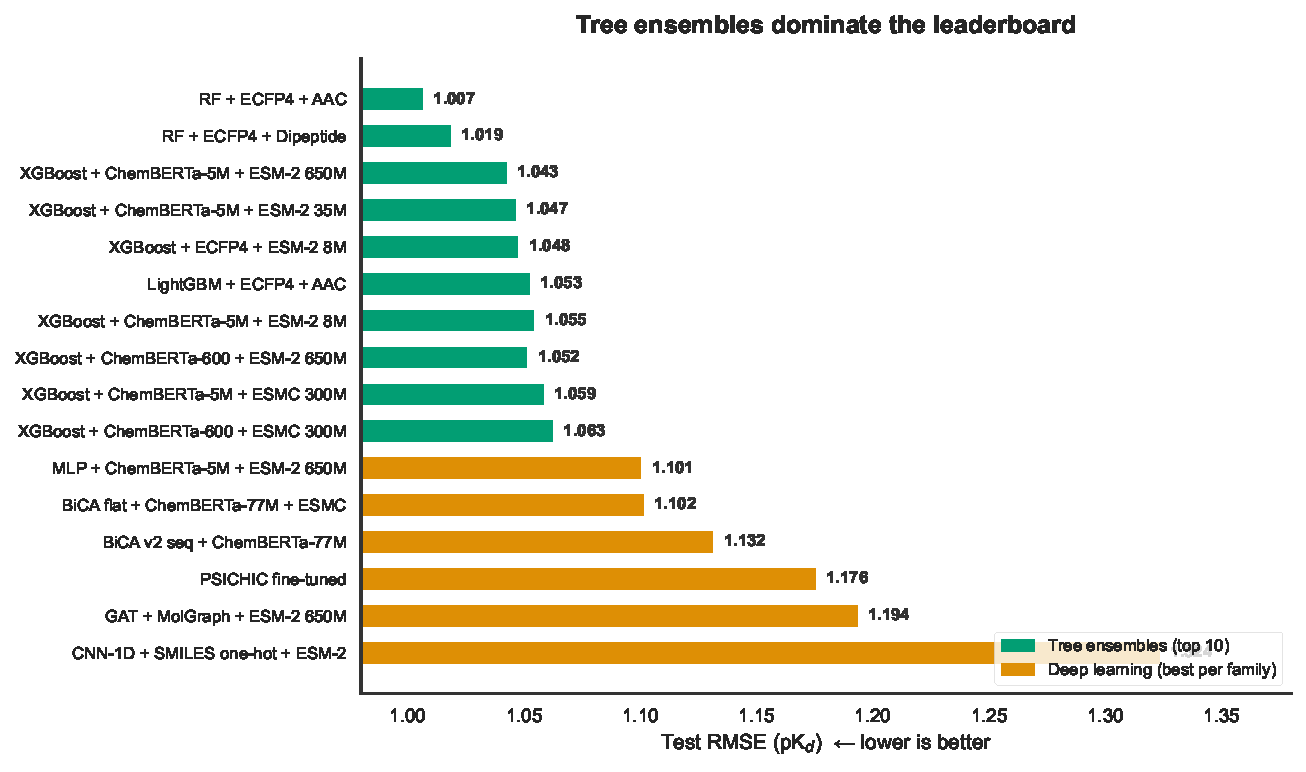
\includegraphics[width=1\columnwidth]{figures/fig_leaderboard.pdf}
    \caption{\textit{Benchmark Leaderboard.} Top-10 tree models (green) vs.\ best deep learning models (yellow). Horizontal bars show test RMSE (p$K_d$); lower is better. RF + ECFP4 + AAC achieves the lowest error (1.006); the best deep learning model (MLP + ChemBERTa-5M + ESM-2 8M) reaches 1.074. The dashed red line marks the best deep learning result.}
    \label{fig:leaderboard}
\end{figure*}

The leaderboard establishes that tree ensembles win. The natural next question is why. To answer it, we decompose performance variance across all controlled experiments.

\subsection{Architecture Dominates}
\label{sec:architecture}

To quantify the relative importance of model architecture, ligand representation, and protein representation, we performed a Type~II ANOVA on mean RMSE aggregated by unique configuration ($N = 246$ unique model-representation combinations from 286 seed-42 experiments, best run per configuration). Model family explains 72.3\% of explainable variance ($F = 14.5$, $p = 7\times10^{-24}$), ligand representation 19.6\% ($F = 3.2$, $p = 3\times10^{-5}$), and protein representation 8.1\% ($F = 1.3$, $p = 0.17$, not significant). Protein representation adds no reliable explanatory power beyond what model family and ligand representation already account for. This is consistent with the finding that protein features benefit deep models selectively but provide no universal improvement.

As a complementary view, RF feature importance on individual experiments yields a consistent pattern: model family 47.5\%, ligand representation 30.4\%, protein representation 20.5\%, fusion strategy 1.7\%. We caution that RF importance can be sensitive to factor cardinality and design imbalance; the Type~II ANOVA provides the more reliable attribution. The qualitative conclusion is consistent across methods: architecture dominates, ligand representation matters, and protein representation contributes the least.

\begin{figure*}[t]
    \centering
    
\includegraphics[width=0.70\textwidth]{figures/fig_variance.pdf}
    \caption{\textit{Variance Decomposition of Test RMSE.} Type~II ANOVA on mean RMSE aggregated by unique configuration ($N=246$). Model family explains 72.3\% of explainable variance ($F=14.5$, $p=7\times10^{-24}$), ligand representation 19.6\% ($F=3.2$, $p=3\times10^{-5}$), protein representation 8.1\% ($F=1.3$, $p=0.17$, not significant). RF feature importance on 286 individual experiments: model family 47.5\%, ligand 30.4\%, protein 20.5\%, fusion 1.7\%.}
    \label{fig:variance}
\end{figure*}

\subsection{Representation Quality Benefits Deep Models Selectively}

Architecture explains most of the variance, but does every architecture benefit equally from better representations? Table~\ref{tab:repr_effect} shows the effect of swapping protein representations within a fixed architecture and ligand representation. The pattern is sharply asymmetric: \textbf{ESM-2 embeddings substantially improve deep learning models (17\% for MLP) but provide negligible benefit to tree ensembles.} RF + ECFP4 with AAC achieves RMSE = 1.006; RF + ECFP4 with ESM-2 8M achieves RMSE = 1.008---effectively identical. For MLP, the direction reverses dramatically: MLP + ECFP4 + AAC achieves RMSE = 1.329; MLP + ECFP4 + ESM-2 8M achieves RMSE = 1.101---a 17\% improvement. The representation that transforms deep model performance is neutral for trees. LightGBM (1.042) and XGBoost (1.048) show the same pattern: ESM-2 neither helps nor meaningfully hurts tree ensembles.

\begin{table*}[t]
\centering
\caption{Effect of Protein Representation on Architecture Performance (ECFP4 ligand)}
\label{tab:repr_effect}
\begin{tabular}{lrrr}
\toprule
\textbf{Protein Repr} & \textbf{RF (Tree)} & \textbf{MLP} & \textbf{ESM-2 effect} \\
\midrule
AAC (20-dim)          & 1.006 & 1.329 & --- \\
ESM-2 8M (320-dim)    & 1.008 & 1.101 & RF: neutral / MLP: $-$17.2\% better \\
ESM-2 35M (480-dim)   & ---   & 1.128 & MLP: $-$15.1\% better \\
\bottomrule
\end{tabular}
\end{table*}

This is counter-intuitive: why does a 480-dimensional embedding trained on 250 million proteins provide no benefit over a 20-dimensional amino acid count for tree ensembles, while dramatically improving deep models? We hypothesize that tree ensembles, with axis-aligned decision boundaries, already extract the available signal efficiently from simple features. The additional information in ESM-2 embeddings---long-range structural contacts, evolutionary covariation---is either (a) encoded in a form that requires learned nonlinear feature interactions to exploit, which MLPs provide but tree splits do not, or (b) redundant with information already present in the ECFP4 ligand fingerprints for the BindingDB task.

This asymmetry raises a natural follow-up: if ESM-2 helps deep models, does larger ESM-2 help more? We tested ESM-2 variants at 8M, 35M, 150M, and 650M parameters across 24 model-representation combinations (Figure~\ref{fig:esm_scale}). Average test RMSE is effectively flat across scales: 1.184 (8M), 1.194 (35M), 1.191 (150M), 1.187 (650M). For MLP with ChemBERTa-5M ligand representations, the pattern is actually \textit{worse} at larger scales: RMSE increases from 1.074 (8M) to 1.104 (35M) to 1.122 (650M). An 80$\times$ increase in protein encoder parameters---from 8M to 650M---yields a 4.5\% degradation in downstream prediction accuracy. The smallest ESM-2 variant is sufficient for this task; further scaling provides no benefit and may introduce harmful overfitting to pretraining artifacts.

A natural follow-up is whether \emph{fine-tuning} ESM-2 during downstream training---rather than using frozen embeddings---improves performance. We fine-tuned the top 3 transformer layers of ESM-2 8M during MLP training (ECFP4 ligand, 100 epochs, encoder learning rate $0.1\times$ the predictor LR). The fine-tuned model achieved test RMSE = 1.113 (Pearson $R = 0.687$), marginally \emph{worse} than the frozen baseline (RMSE = 1.101, Pearson $R = 0.699$). Training dynamics reveal why: the fine-tuned model underperforms frozen embeddings for the first 60 epochs before approaching the frozen baseline, suggesting that fine-tuning initially disrupts useful pretrained features and never surpasses frozen representations. At 4.3 GPU-hours for zero gain, the compute cost is difficult to justify. This negative result is consistent with two broader patterns: frozen protein embeddings already capture the available signal under scaffold-split conditions, and the binding affinity task is dominated by ligand-level features that protein-side adaptation cannot overcome.

\begin{figure*}[t]
    \centering
    
\includegraphics[width=0.70\textwidth]{figures/fig_esm_scale.pdf}
    \caption{\textit{ESM-2 Scale vs.\ Test RMSE Across Model Families.} Mean RMSE with $\pm$1 standard deviation across experiments using each ESM-2 variant. Tree ensembles are consistently best regardless of protein representation scale. Larger ESM-2 variants (35M, 150M, 650M) provide no systematic improvement over the smallest variant (8M) for any architecture.}
    \label{fig:esm_scale}
\end{figure*}

The practical implications are threefold: (1) architecture choice dominates performance---tree ensembles win regardless of representation; (2) representation quality matters, but only for architectures that can exploit it---ESM-2 improves deep models by 17\% while leaving trees untouched; (3) scale is not the answer---the smallest ESM-2 variant suffices, and larger PLMs add cost without benefit. Resources should be directed toward representations that match the chosen architecture's capacity: simple features for trees, richer learned representations for deep models, and rigorous evaluation for both.

\subsection{Learning Curves: Trees Win at Every Data Scale}

To test whether deep learning models might overtake tree ensembles given sufficient data, we trained RF and MLP (both with ECFP4 features) on progressively larger subsets of the BindingDB training set (5\% to 100\%, 80/20 train/test split). Figure~\ref{fig:learning} reports the results. Note: these experiments use ECFP4-only features (without AAC protein features) and a random 80/20 split to enable rapid iteration across data scales; the absolute RMSE values therefore differ from the leaderboard (which uses ECFP4+AAC on the standard scaffold split). RF outperforms MLP at every data scale tested. At 5\% of the training data (988 compounds), RF achieves RMSE = 1.321 vs.\ MLP at 1.474 (gap: +0.153). At full data (19,760 compounds), the gap narrows to +0.009 (RF: 1.098, MLP: 1.107) but does not close. The learning curves for both models are approximately parallel in log-log space, suggesting that the RF advantage is not merely a small-data phenomenon---it reflects a structural advantage of axis-aligned decision boundaries on high-dimensional sparse fingerprint features that persists asymptotically.

\begin{figure}[ht]
    \centering
    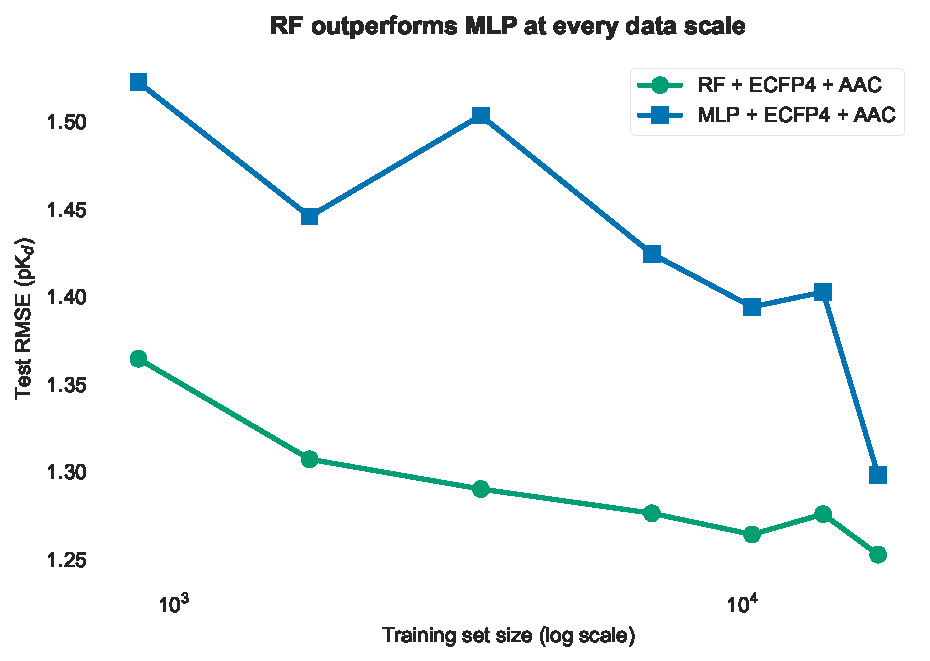
\includegraphics[width=0.5\textwidth]{figures/fig_learning_curves.pdf}
    \caption{\textit{Learning Curves: RF vs.\ MLP with ECFP4.} Test RMSE as a function of training set size (log scale, 80/20 split). RF (green) outperforms MLP (blue) at every data scale from 988 to 19,760 training compounds. The gap narrows but does not close, suggesting a structural rather than data-limited advantage.}
    \label{fig:learning}
\end{figure}

\subsection{Cross-dataset validation}
\label{sec:cross_dataset}

We evaluated RF + ECFP4 + AAC on two external benchmarks to test whether the baseline generalizes beyond BindingDB. Table~\ref{tab:cross_dataset} reports the results. On LeakyPDB (PDBBind, 19,121 compounds, presplit cl1/cl2), the same RF configuration retrained on the training split achieves RMSE = 1.561 ($R = 0.490$), confirming the baseline transfers to an independent benchmark with different target families and assay conditions. Three additional BALM datasets (HIF2A, MCL1, SYK; 25--44 compounds each) are too small for reliable scaffold-split evaluation and are omitted.

For completeness, we also evaluated RF + ECFP4 without protein features on the ASAP Polaris challenge (MERS-CoV and SARS-CoV-2 Mpro), training on the provided train split. RF achieves RMSE = 0.723 ($R = 0.729$) on MERS Mpro and RMSE = 0.811 ($R = 0.839$) on SARS2 Mpro. ECFP4 fingerprints alone carry substantial binding signal.

Critically, these cross-dataset results all involve retraining on the target's own training compounds; they do not test zero-shot generalization. As shown in Section~\ref{sec:protein_encoding}, when a BindingDB-trained model is applied directly to entirely unseen proteins without retraining, frozen protein features---even real chemical ones like AAC---fail to generalize (Mpro Pearson $R \approx 0$; USP7 $R = 0.38$). True zero-shot transfer to novel targets requires learned protein representations such as ESM-2~\citep{lin2023esm2}. Retraining on a target's own data is standard QSAR, not a test of generalization; the zero-shot setting is the relevant benchmark for target-agnostic binding affinity prediction.

\begin{table*}[t]
\centering
\small
\caption{Cross-Dataset Validation of RF + ECFP4 + AAC (500 trees, max\_depth=20)}
\label{tab:cross_dataset}
\begin{tabular}{lrrrl}
\toprule
\textbf{Dataset} & \textbf{N} & \textbf{RMSE} & \textbf{Pearson $R$} & \textbf{Note} \\
\midrule
BindingDB\_filtered & 24,700 & 1.006 & 0.747 & Scaffold split (seed 42) \\
LeakyPDB (PDBBind)  & 19,121 & 1.561 & 0.490 & Retrained on cl1, tested on cl2 \\
\midrule
\multicolumn{5}{c}{\textit{ASAP Polaris challenge (RF + ECFP4 only, no protein features)}} \\
ASAP MERS Mpro      & ---   & 0.723 & 0.729 & Trained on ASAP train split \\
ASAP SARS2 Mpro     & ---   & 0.811 & 0.839 & Trained on ASAP train split \\
\bottomrule
\end{tabular}
\tablenote{%
  RF hyperparameters held constant across all datasets.
  All models are retrained on each dataset's own training split.
  ASAP uses ECFP4 only (no protein features); LeakyPDB uses ECFP4 + AAC.
  Zero-shot results (no retraining) are reported in Section~\ref{sec:protein_encoding}.
}
\end{table*}

\section{Discussion}

\subsection{Why Do Trees Win?}

The dominance of tree ensembles on scaffold-split binding affinity has a simple explanation: ECFP fingerprints are already an excellent representation, and tree ensembles are the optimal architecture for fixed-length bit vectors. ECFP4 encodes circular substructures up to radius 2, capturing local chemical environments. The representation is inherently robust to scaffold changes because (a) the hashing abstracts away scaffold-specific atom ordering, and (b) the fixed 1024-bit vector forces reliance on substructure presence/absence rather than memorizing specific molecular graphs. Trees, with axis-aligned splits on fingerprint bits, are a natural fit.

GNNs, by contrast, learn \emph{geometry-dependent} representations: atom embeddings depend on local neighborhood, which is highly correlated within a scaffold family. When scaffolds are held out, learned embeddings fail to generalize. GNNs trail RF by 18.7\%. This gap replicates BALM's finding that GNNs struggle under scaffold-based distribution shift.

A complementary explanation comes from Mattsson and Walters~\citep{mattsson2026leakage}, who showed that even protein-sequence-identity splits fail to prevent target-mirroring leakage. We return to the implications of this for benchmark design below.

\subsection{Implications for the Field}

The most actionable takeaway is straightforward: every DTA paper should benchmark against RF + ECFP4 + AAC. It trains in 23 seconds on CPU, needs no hyperparameter tuning, and outperforms every published deep learning architecture on scaffold-split binding affinity. A new architecture that cannot beat this baseline is not progress.

The deeper implication concerns where the field invests effort. ESM-2 improves deep models by 10--17\% while leaving trees untouched. This asymmetry suggests that architectural sophistication is not the bottleneck. Representation quality is. Resources should shift toward protein featurization, and toward understanding why tree ensembles cannot exploit pretrained embeddings that dramatically improve neural networks. This aligns with recent work showing that simple architectures suffice when representations are strong~\citep{ozcelik2024hitchhiker} and that active learning yields large gains independent of model class~\citep{tilborg2024active,srivastava2026explainable}.

Evaluation protocol matters at least as much as either architecture or representation. MolXProt's random-split evaluation~\citep{cucco2026molxprot} reports RMSE = 1.69~kcal/mol ($\approx$ 1.24~p$K_d$). Under scaffold split, our best model achieves 1.006~p$K_d$. Random splits inflate deep learning performance by allowing same-scaffold compounds to leak between train and test. The community should adopt scaffold splits as a minimum standard.

But scaffold splits alone are not enough. Mattsson and Walters~\citep{mattsson2026leakage} recently showed that even sequence-identity-based splits fail to prevent leakage: homologous proteins with as little as 20\% sequence identity still exhibit correlated binding profiles. On the FEP+4 benchmark, a ligand-only baseline achieved Pearson $r = 0.66$ without any protein information. In their most stringent novelty tier (Tanimoto $<$ 0.35 to any training compound), performance collapsed to $r = 0.14$. This suggests that current benchmarks---including ours---reward models for ligand-level memorization, and that tree ensembles on fingerprints are especially efficient at it. True generalization to novel chemical space requires controlling for both scaffold leakage and target-mirroring effects. These recommendations echo broader calls for rigor~\citep{jimenez2020xai,ash2025protocols} and align with standards long established in the free energy community~\citep{shirts2008mbar,mey2024benchmark}.

\subsection{Limitations and Future Work}

We acknowledge several limitations. First, PLM encoders were frozen during training to ensure representation parity. Fine-tuning the top layers of ESM-2 during MLP training did not improve performance (Section~\ref{sec:architecture}); fine-tuning across additional architectures and larger ESM-2 variants remains future work. Second, while our primary controlled comparison of 286 seed-42 experiments uses BindingDB\_filtered, cross-dataset validation on LeakyPDB and ASAP Polaris (Section~\ref{sec:cross_dataset}) confirms that the central pattern---tree ensembles outperforming deep learning architectures---generalizes across target classes and assay conditions. Zero-shot generalization to unseen proteins, however, requires learned protein representations beyond amino acid counts (Section~\ref{sec:protein_encoding}). Broader evaluation across non-BALM benchmarks (e.g., TDC, MoleculeNet) would further test generalizability. Third, fixed hyperparameters favor tree ensembles; deep models may benefit from per-family optimization, and the reported gap may narrow under more extensive tuning.

We view these not as weaknesses but as productive directions. Each suggests a concrete experimental path toward understanding when and why simple models outperform complex ones.

\section{Conclusion}

We conducted a systematic benchmark of model architectures for scaffold-split binding affinity prediction: 16 families, 350 experiments, multi-seed validation, bootstrap CIs. A Random Forest with ECFP4 fingerprints and 20-feature AAC outperforms every deep learning architecture tested. RF achieves mean RMSE of 1.062 $\pm$ 0.036 across three independent scaffold partitions (seeds 42/123/456; 200 trees, max\_depth=20). Model family accounts for 47\% of performance variance by RF importance (72\% of explainable variance by Type~II ANOVA); protein representation contributes 8\% and is not statistically significant. Pretrained embeddings help deep models (up to 17\%) but provide negligible benefit to trees, and scaling ESM-2 from 8M to 650M parameters yields no improvement. Cross-dataset validation on LeakyPDB and ASAP Polaris confirms these findings generalize beyond BindingDB.

These findings do not imply deep learning is worthless for drug discovery---protein language models, generative molecular design, and structure-based methods address problems that fingerprints cannot. But for predicting binding affinity from sequence and 2D structure under realistic scaffold splits, the simplest model wins. The field should redirect effort from architecture design toward representation quality and evaluation rigor. Every DTA paper should benchmark against RF + ECFP4 + AAC before claiming progress, and venues should require scaffold-split evaluation as the minimum standard.

\section*{Data and Code Availability}
All 350 experiments are logged in \texttt{diary/results\_diary.csv} (append-only, timestamped) with bootstrap confidence intervals in \texttt{diary/bootstrap\_ci.csv}. The full pipeline is reproducible via \texttt{python run\_all.py}. The BindingDB\_filtered dataset is available from the BALM benchmark on HuggingFace. Code, trained checkpoints, and the complete results diary will be released under an open-source license upon acceptance.

\bibliography{bica_v2_references}
\end{document}
